\documentclass[10pt]{article}
\usepackage[a4paper,margin=17mm]{geometry}
\usepackage[T1]{fontenc}\usepackage{lmodern,amsmath,amssymb,booktabs,graphicx,hyperref}
\hypersetup{colorlinks=true,urlcolor=blue}\setlength{\parindent}{0pt}\setlength{\parskip}{5pt}
\newcommand{\rec}{\texttt{uniform-20261029}}
\sloppy\setlength{\emergencystretch}{3em}
\begin{document}
\begin{center}{\Large Attempt02: positive replay, incomplete control contract}\\2026-10-29; uniform-20261029\end{center}
At input \texttt{42b72c3a2feb}, the corrected independent audit passes96 arms,
896 source recoveries,210 comparisons,536 states and172 failed recovery queries.
Joint original/reduced counts are0/0. The runner exits2: false-row replaced an
already empty first row list by empty, so the changed-payload guard correctly
rejects a no-op. No successful control rejection/backend completion is claimed.
Versioned v3 finds an actual nonempty query and removes one real row; this was
compiled and committed at \texttt{0e88deaae36a} before a full third execution.
The original v2 source/payload remain. All97 producer files and the positive
receipt match the final successful run byte for byte. The full record retains
all policies/losses; the graph below shows the same audited response profiles.
\par
\noindent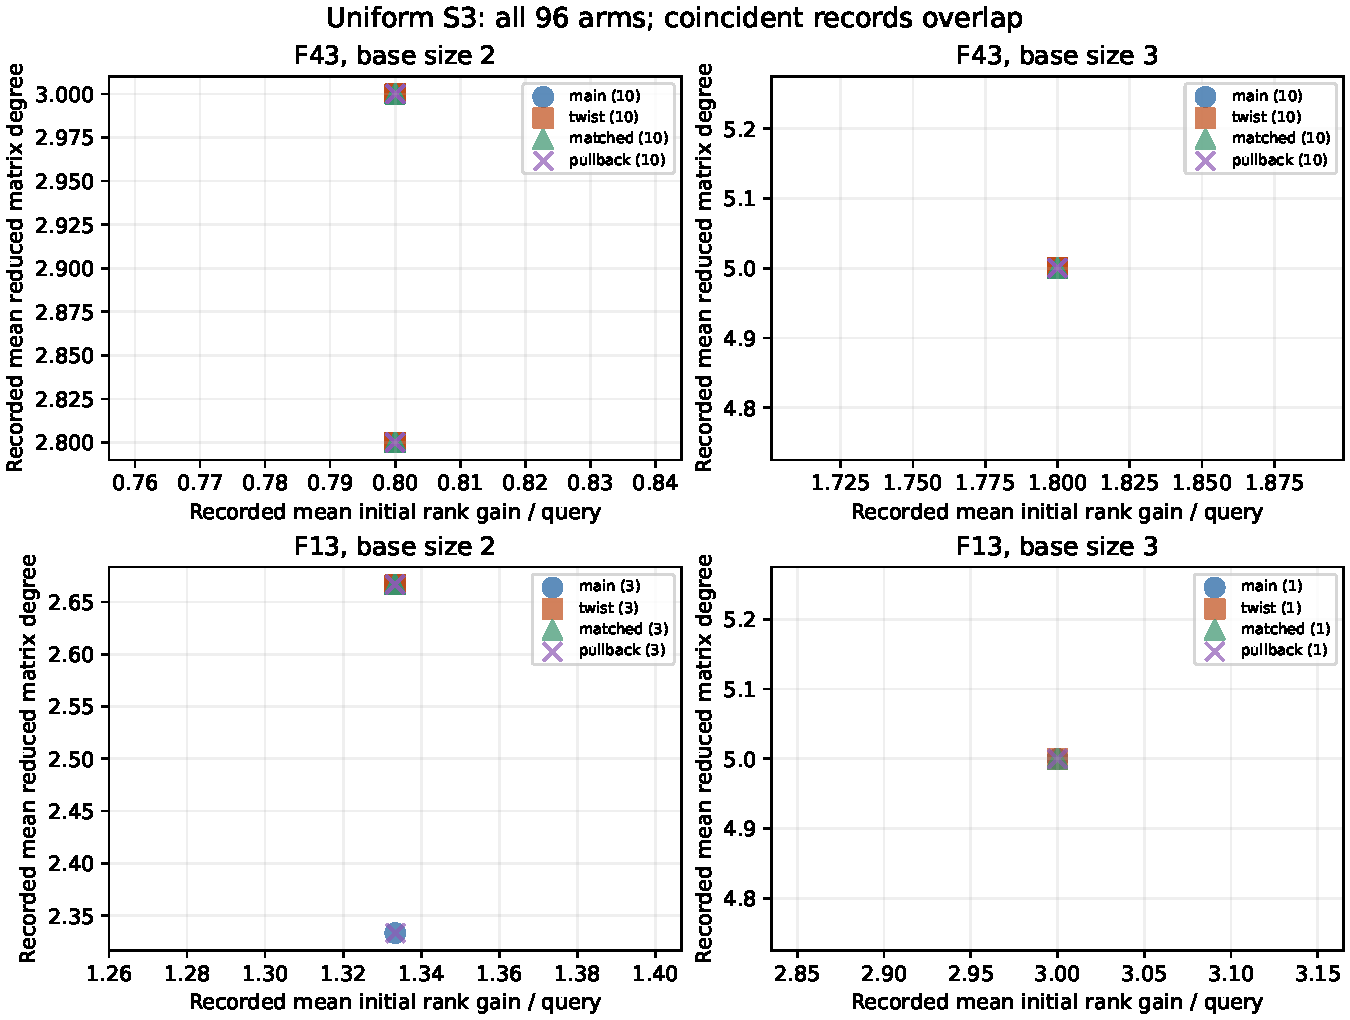
\includegraphics[width=.78\linewidth]{../profiles.pdf}

\textbf{Execution contract.} Same full preregistered96/896/210 workload, deterministic
response census, existing local host/two workers,600s command caps, no clock or
speed claim. Raw inputs/commands/exits and precise failed payload are restored by
\path{validation/uniform-20261029/restore-runs.sh}. The official checkpoint gate
passed before this scientific execution. No private key/token enters the record.

\textbf{Source links.} \path{UNIFORM_YIELD_20261025_PROTOCOL.md}, dated
audit/control correction contracts, and final \path{reports/uniform-20261029/README.md}.
The broader useful-yield/degree/source-DLP objective remains open.
\end{document}
